\chapter{METHODOLOGIES}

\graphicspath{ {./methodologies/} }
%%%%%%%% This line gets rid of page number on first page of text
\thispagestyle{empty}

%%%%%%%%%%%%%

\section{Method Selection}

The methodologies section covers methods chosen to investigate the research problem. We begin this section by restating our research problem and underlying assumptions underpinning our study: interpreting and understanding deep neural networks using interactive visualization, to inspire human curiosity and learning among the non-technical audience, as well as broaden people's access to interactive tools for deep learning.

\subsection{Scientific Methods}

The primary method selected for the research process is the scientific method. We selected this method as it involves careful observation and empirical study.

As deep learning is essentially a method for machines to learn from data and classifying patterns that is loosely modeled on the way a biological brain learns to solve problems. The scientific method is aptly suited for this type of research as it involves careful observation and empirical study of the topic in question, which includes rigorous skepticism about what is observed and iterative testing and experimentation to validate or invalidate it.

The underlying principles of the scientific method \cite{gauch_jr_2012} are essential for evaluating the hypothesis, enhancing perspective, increasing productivity, and inspiring innovation. These principles include logic, probability, parsimony and hypothesis testing, as well as science's presuppositions, limitations, principles and bold claims of rationality and truth. Beyond such methodology, some practical issues are shared broadly across the sciences, such as implementing effective science education and relating the scientific enterprise to the humanities.

The scientific method consists of two stages \cite{2016397}: the first consists of formulating hypotheses, and the second consists of testing them. What differentiates this from other forms of methods is the second stage: subjecting hypotheses to empirical testing by ascertaining whether or not predictions derived from hypotheses are borne out in relevant observations and experiments. Hypotheses and assumptions are the initial stages of scientific inquiry because they incentivize seeking truth and a hint as to where to find it. \cite{AYALA2016xi}

Additionally, we also employed other research methods to bolster our research processes, such as action as research, agile development and system design. The selection of a research methodology was dependent on the research question itself and how best it can be addressed: interpreting deep neural networks.

\subsection{Action Research}
Action Research is a research methodology driven by practical problems, emphasis participatory research, and develops practically useful solutions to a real-world problem iteratively. It offers a systematic, collaborative approach to conducting research that satisfies both the need for scientific rigor and promotion of sustainable social change and has been taken up by a variety of researchers in both academic and industrial settings. \cite{Hayes:2011:RAR:1993060.1993065}

Action Research emphasizes the knowledge produced in the context of the application (Lewin, 1946; Susman \& Evered, 1978). It’s a distinct candidate research method when the objective is to explore theory concerning practice.

\section{Research Hypothesis}

While deep neural networks learn efficient and powerful representations, they are often considered a ‘black-box.’ In most cases, they learn representation that is difficult to extract and present in a human-readable form. While it can be true for certain types of deep learning models, it is not entirely true for some of the popular networks like a convolutional neural network, recurrent neural network, semi-supervised and unsupervised method.

\section{Hypothesis Testing}

<REWRITE> Building upon our research question stated in the above section; we formulated our hypothesis as follows -  Develop a prototype that serves a set of utilities or toolkit for interpreting a visual classifier by providing visual evidence for their decision using interactive visualization.

\section{Prototype Objective}

<REWRITE> The prototype is intended and designed for people with a non-technical background to understand the fundamental concepts of the neural network, in our case, a visual classifier. Our objective can be summarized mainly as (1) Explanation of neural networks for people with a non-computer science background (2) Inspire curiosity and learning among non-technical audiences  (3) Broadens people's access to interactive tools for deep learning.

\section{Technical Design}
The following segment provides an overview of the technical design and resources required for the successful development of the prototype. It provides a high-level overview of the components in scope, functionality, dataset and environmental setup.

\subsection{Model Selection}

<REWRITE> As model selection is the centerpiece of the data science workflow, we evaluated a set of candidate pre-trained models by running a series of the experiment. It mainly helped us assess if the data collected is well suited to the problem of model selection. We also considered the hyperparameter setting and other configuration details required to fit the model. We also tested the compatibility of the model with the available public dataset. Based on our evaluation we selected VGG-16 as the primary model for the prototype development. This model is trained on the imagenet database.

VGG-16 is based on convolutional neural network model proposed by the Visual Geometry Group from the University of Oxford in the paper “Very Deep Convolutional Networks for Large-Scale Image Recognition”.  The model achieves 92.7\% top-5 test accuracy in ImageNet, which is a dataset of over 14 million images belonging to 1000 classes. It was one of the famous model submitted to ILSVRC-2014 competiton. This is used as the backbone network in our project.

A schematic view of Visual Geometry Group 16 Model.~\ref{fig:CNN-1}.
\begin{figure}[htbp]
\centering
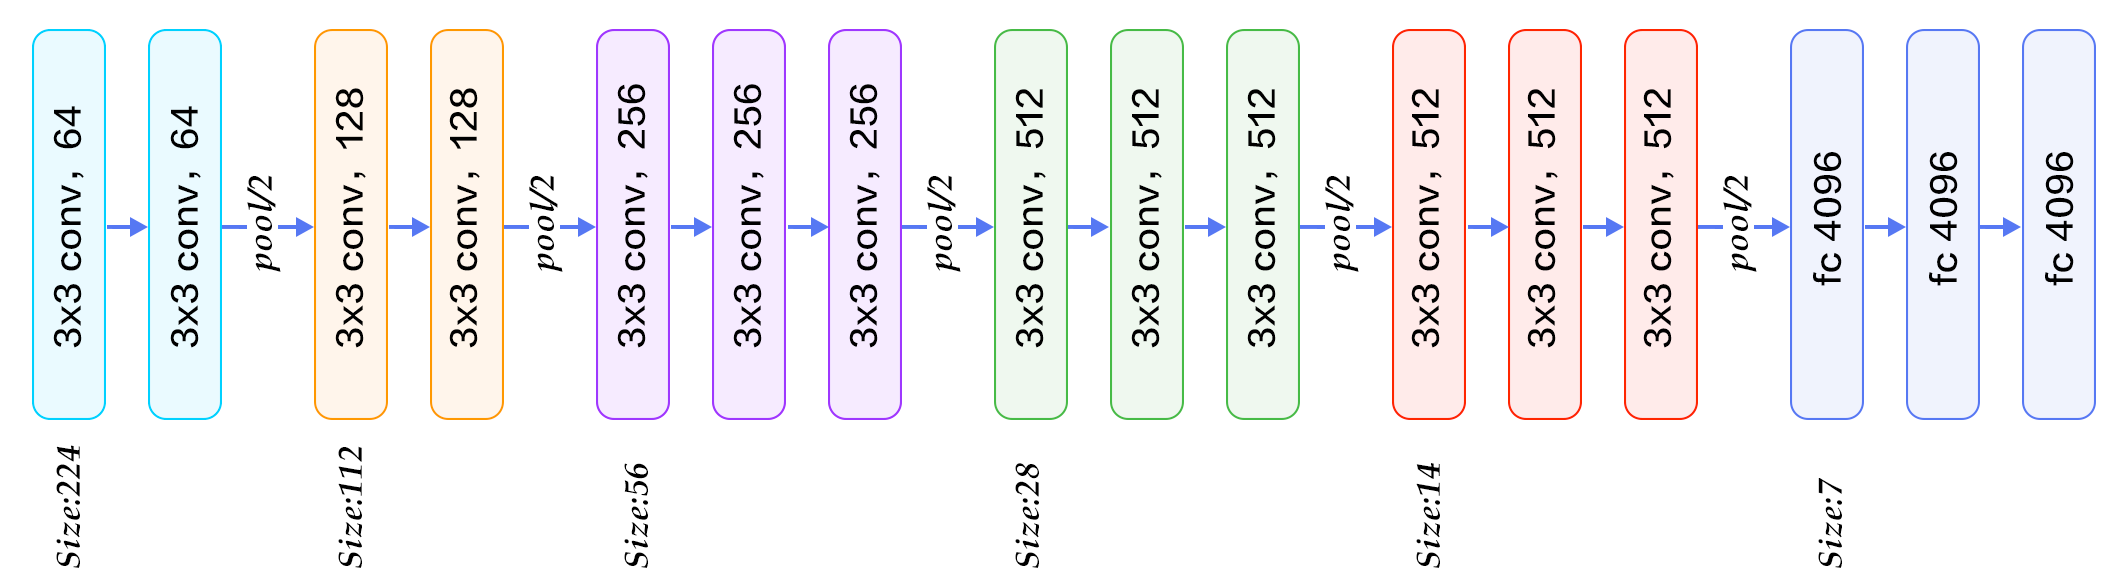
\includegraphics[width=1\textwidth]{images/cnn-vgg16-1.png}
\caption{VGG16 hidden layers}
\label{fig:CNN-1}
\end{figure}

\subsection{Dataset}

ImageNet database consist of over 15 million labeled high-resolution images that belong to roughly 22,000 categories. These images were downloaded from Google image search and labeled by humans using Amazon's Mechanical Turk crowd-sourcing tool in 2012. It took about two and half years to label all the images. The labeled dataset was first introduced in a competition called the ImageNet Large-Scale Visual Recognition Challenge (ILSVRC). The competition used a subset of ImageNet with around 1000 images in each of 1000 categories. In total, there are 1.2 million training images, 50,000 validation images, and 150,000 testing images. To maintain consistency of resolution, images have been down-sampled to a fixed resolution of 256x256 dimensions.
    
\subsection{Framework Selection}

<REWRITE> To develop client-side deep learning application, we surveyed several open source machine learning framework for the web such as TensorFlow, Keras, PyTorch, Caffe and WebDNN. Based on our assessment and feedback from the developer community, we found TensorFlow.js as a right choice for training and inference of deep learning models on the browser. Additionally, Tensorflow.js is feature-rich and takes advantage of GPU-accelerated training processes. 

<REWRITE> We use TensorFlow and TensorFlow.js library, released by Google in Mar. 2018 is an in-browser open source machine learning framework that supports defining, training and running deep learning models in the browser using JavaScript (JS). It is the successor of the deeplearn.js which is now called TensorFlow.js Core. 

<REWRITE> While several other open source JS platforms for machine learning have appeared in recent past, to our knowledge, TensorFlow.js is commonly used and have enabled developers to create interactive and explorable explanations for deep learning models on the web.

<REWRITE> TensorFlow.js leverages GPU processing power to accelerate deep learning tasks on browsers via WebGL. WebGL is a back-end compute on GPU by WebGL API, which is a JavaScript API for rendering interactive 2D and 3D graphics within any modern compatible browsers. TensorFlow.js provides a low-level core API to perform linear algebra operations and automatic differentiation, and high-level Layers APIs for building and training models. The layers used in Tensorflow.js support the Tensorflow and Keras layers in the native platform. Supported features also include conversion of models built in the native platform, importing pre-trained models for inference and retraining imported models.

\subsection{Visual Exploration Tool}

DeepViz is a visual exploration tool targeted towards the non-technical audience to explore the inference (or predictions) made by a visual classifier, an image recognition deep learning model.

Deep learning in the browser is at the experimental stage and recently a bunch of JavaScript-based deep learning framework has been introduced, making it possible to perform several deep learning tasks directly on the browser. Some of the supported features include model training, importing pre-trained models, transfer learning and inferences.

However, there is a debate on the feasibility and effectiveness of the web-based deep learning applications. One one hand, those who object think browsers are not primed for running deep learning tasks and its merely impractical due to the poor performance of client-side scripting and limitations imposed by the browsers. 

On the other hand, advocates think that the browser is an ideal platform for realizing client-side machine learning that allows highly rich interaction and improves personalization for end users. The benefits include but not limited to faster user interaction, preserving data privacy, lower back-end payload, reduced data transfer and performance latency of HTTP client-server communication.

\section{Computational Environment}

\subsection{Client-side Neural Network Overview}
Developing AI applications using modern deep learning framework is a non-trivial task. Normally these frameworks and libraries are leveraged by native applications that run on a native platform environment such as Linux, Windows, MacOS/iOS and Android. Thus most production-level libraries are developed for and written in Python, Java and C++. 

Developing AI application that is cross-platform and portable on multiple devices is not easy. The development of a native application is an intricate and time-consuming process. It is particularly complicated for mobile applications as the app vendors usually need to develop and maintain both iOS and Android version, in addition to the desktop application.

Compared to the native application, client-side applications can make the portability issue simpler for the cross-platform. The sample implementation of deep learning powered web application can be deployed on multiple platforms regardless of operating systems, hardware or device types.

\subsection{Supported Browser Features}
We analyzed the supported browser features for machine learning tasks and taken into consideration the factors that may affect the efficiency when building and deploying deep learning application on the web. One of them is the debugging capability to support model and data inspection when running deep learning tasks.

Further, in-browser deep learning allows users to use their local data and then train the model directly in the browser, which means there is no back-end end or server is necessary. 

\section{Experimental Setup}

We set up the development environment for building the client side application using JavaScript ES6, Node.js and Tensorflow.js. We download the required modules and dependencies, including tensorflow.js, D3, transpiler to convert code written in JavaScript ES6 into plain old ES5 JavaScript that can run in any browsers. We use Webpack and Bitbucket for bundling and deployment.

\iffalse
\section{Infrastructure and Tooling}
\subsection{GPU Acceleration}
\subsection{Hardware}
\subsection{Software}
\subsection{Build and Tooling}
\subsection{Cloud computing services}

\subsection{Base Architecture}
\subsection{Model Conversion}
\subsection{Dataset}
\subsection{Data Pre-processing}
\subsection{Parameter Settings}
\subsection{Application Prototype}
\subsection{Real-time processing}
\fi